\chapter{Odoo Sous Docker}

	Dans ce qui suit, nous allons donner une idée sur l'interface que fournit Docker pour la provision des services (conteneurs). Nous allons réalisé la mini-architecture suivante:
	
	\begin{figure}[H]
	\centering
	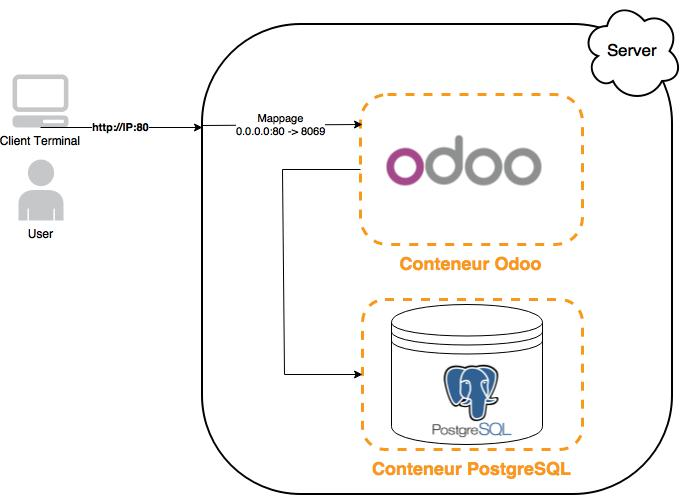
\includegraphics [scale=0.5]{biblio/odoo.jpg}
	\caption{Odoo sous Docker}
	\label{fig:}
	\end{figure}

\section*{Environnement technique}
	
	On va partir d'un serveur Ubuntu 14.04-64 bits avec Docker installé (L'installation ne sera pas détaillé), ou de préférence, un serveur CoreOS où Docker est déja inclut avec ce système d'éxploitation. A noter que Docker nécéssite un linux 64 bits avec un noyau >= 3.8.


\section*{Installation de PostgreSQL}

	Odoo a besoin d'un serveur de base de donnée PostgreSQL, la commande suivante permet de l'installer:

	\begin{lstlisting}[caption=Installation de PostgreSQL]
		$ docker run -d -e POSTGRES_USER=odoo -e POSTGRES_PASSWORD=odoo --name db postgres
	\end{lstlisting}




\section*{Installation d'Odoo}

	L'installation d'Odoo se fait grâce à la commande suivante:
	\begin{lstlisting}[language=bash,caption=Installation d'Odoo]
		$ docker run -p 80:8069 --name odoo --link db:db -t odoo
	\end{lstlisting}

	En quelques secondes, on pu lancer le service Odoo prêt à être utilisé, personnalisé, et éventuellement porté vers un autre serveur. Pour accéder au service il suffit de taper dans le navigateur:

	\begin{lstlisting}[language=bash]
		http://IP_SERVEUR:80
	\end{lstlisting}

	




\chapter{Docker-compose}

	On va réaliser l'installation détaillé dans \emph{l'Annexe A} avec l'outil \emph{Docker-compose}. Cet outil permet de définir dans un fichier \acrshort{yaml} l'architecture de l'application. Enfin, on peut faire des manipulation (démarrage, redémarrage, arrêt) sur toute l'architecture comme si c'était un seul service.

	\begin{lstlisting}[language=bash,caption=Installation d'Odoo avec Docker-compose]
		odoo:
	  		image: odoo
		  	links:
		   		- db
		  	ports:
		   		- "80:8069"
		db:
		  	image: postgres
		  	environment:
  				- POSTGRES_USER: odoo
  				- POSTGRES_PASSWORD: odoo
	\end{lstlisting}

	\begin{lstlisting}[language=bash,caption=Lancement d'Odoo avec Docker-compose]
		$ docker-compose up -d
	\end{lstlisting}


\chapter{Installation du superviseur}
	
	Voici les fichiers d'installations de cAdvisor, InfluxDB, Heapster et Grafana. On va les charger dans le cluster puis les installer un à la suite de l'autre.

	\begin{lstlisting}[language=,caption=cadvisor.service]
		[Unit]
		After=docker.service
		Requires=docker.service
		[Service]
		Restart=always
		ExecStartPre=/usr/bin/docker pull google/cadvisor:latest
		ExecStartPre=-/bin/bash -c "docker inspect cadvisor >/dev/null 2>&1 && docker rm -f cadvisor || true"
		ExecStart=/usr/bin/docker run --volume=/var/run:/var/run:rw --volume=/sys/fs/cgroup/:/sys/fs/cgroup:ro --volume=/var/lib/docker/:/var/lib/docker:ro --publish=8080:8080 --name=cadvisor google/cadvisor:latest
		ExecStop=/usr/bin/docker rm -f cadvisor
		[X-Fleet]
		Global=true

	\end{lstlisting}

	\begin{lstlisting}[language=,caption=influxdb.service]
		[Unit]
		After=docker.service
		Requires=docker.service
		Rquires=docker_configs.mount
		[Service]
		ExecStartPre=-/usr/bin/docker kill influxdb
		ExecStartPre=-/usr/bin/docker rm influxdb
		ExecStartPre=/usr/bin/docker pull kubernetes/heapster_influxdb:v0.3
		ExecStart=/usr/bin/docker run -p 8083:8083 -p 8086:8086 -v /data/influxdb:/data --hostname="influxdb" --name influxdb kubernetes/heapster_influxdb:v0.3
		ExecStop=/usr/bin/docker stop nodejscluster
		TimeoutStartSec=0
		Restart=always
		RestartSec=5s

	\end{lstlisting}

	\begin{lstlisting}[language=,caption=heapster.service]
		[Unit]
		After=docker.service
		After=influxdb.service
		Requires=docker.service
		Requires=influxdb.service
		[Service]
		TimeoutStartSec=0
		ExecStartPre=-/usr/bin/docker kill heapster
		ExecStartPre=-/usr/bin/docker rm heapster
		ExecStart=/bin/bash -c "HOST_IP=`getent hosts %H|/usr/bin/cut -d\" \" -f1`; /usr/bin/docker run --name heapster --link influxdb:influxdb kubernetes/heapster:v0.13.0 --source=\"cadvisor:coreos?fleetEndpoint=http://$HOST_IP:4001&cadvisorPort=8080\" --sink='influxdb:http://influxdb:8086'"
		Restart=always
		RestartSec=5
		ExecStop=/usr/bin/docker stop heapster
		[X-Fleet]
		X-ConditionMachineOf=influxdb.service
	\end{lstlisting}

	\begin{lstlisting}[language=,caption=grafana.service]
		[Unit]
		After=docker.service
		After=influxdb.service
		Requires=docker.service
		Requires=influxdb.service
		[Service]
		TimeoutStartSec=0
		ExecStartPre=-/usr/bin/docker kill grafana
		ExecStartPre=-/usr/bin/docker rm grafana
		ExecStart=/usr/bin/docker run --name=grafana --link influxdb:influxdb -p 8090:8080 -e INFLUXDB_HOST=influxdb kubernetes/heapster_grafana:v0.7
		Restart=always
		RestartSec=5
		ExecStop=/usr/bin/docker stop grafana
		[X-Fleet]
		X-ConditionMachineOf=influxdb.service
	\end{lstlisting}	

	\begin{lstlisting}[language=bash,caption=Lancement des services]
		$ ssh core@104.154.75.6 
		$ fleetctl load cadvisor.service
		$ fleetctl start cadvisor.service
	\end{lstlisting}



\chapter{Installation de la PaaS Deis}

\chapter{Douzes-éléments d'un SaaS}


Dans l'informatique moderne, le logiciel est généralement livré comme un service: appelés \acrshort{saas}. Les douzes-éléments d'un SaaS est une méthodologie pour la création d'application qui:

\begin{itemize}
	\item Réduit le temps et le coût pour les nouveaux développeurs participant au projet;
	\item offre une \textbf{portabilité maximale} entre les environnements d'exécution;
	\item Sont appropriées pour le \textbf{déploiement} sur les \textbf{plates-formes de cloud} modernes, éliminant ainsi la nécessité de serveurs et d'administration de systèmes;
	\item \textbf{Réduit la divergence} entre le développement et la production, permettant un déploiement continu;
	\item peut \textbf{monter en charge} sans toucher aux outils, à l'architecture, ou à les pratiques de développement.
\end{itemize}


La méthodologie des douzes-éléments synthétise l'éxpérience de l'équipe de Heroku, un des tout premiers services cloud \cite{12-factors}. Elles peut être appliquée à des applications écrites dans n'importe quel langage de programmation, et qui sont combinées à n'importe quel services (base de données, file d'attente, mémoire cache, etc.).


\section*{code source}

Le code source de l'application doit être unique mis et suivi depuis un système de contrôle de version comme Git.

\section*{Dépendances}

La plupart des langages de programmation un sytème de gestion de dépendances. Ainsi, une application doit déclarer explicitement et isoler les dépendances. Un SaaS robuste ne repose jamais sur l'éxistence implicite des dépendances. 

\section*{Configuration}

Les variables de configurations peuvent varier entre les environnements (développement, test, production, etc). Ces variables ne doivent jamais être stockées dans des constantes à l'intérieur du code. Une bonne pratique c'est les stocker dans des variables d'environnement.

\section*{title}



\section*{Build, release, run}
\section*{Processus}

Les processus d'une application doivent être \textbf{sans état} (stateless). Les données persistentes doivent être stockées dans une base de donnée.

\section*{Attachement de port}

Chaque service doit être exporté via un port.

\section*{Concurrence}


\section*{Jetable}

Les processus d'une application sont jetables, ils peuvent être stoppés ou démarrés à n'importe quel moment rapidement et sans causer de problèmes.

\section*{Parité Dev/Prod}

Il faut garder tous les environnements (développement, test, production, etc) similaires.

\section*{Messages logs}

Les messages logs sont très importants, il faut les traiter comme des flux d'événements.

\section*{Processus admin}